\documentclass{article}
\usepackage{tikz}
\usetikzlibrary{shapes.geometric}

\begin{document}

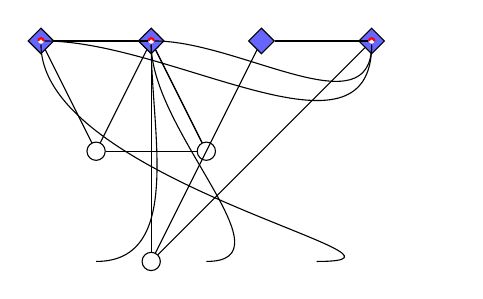
\begin{tikzpicture}[scale=0.7,transform shape]
    \node[draw,circle] (v1) at (0,0) {};
    \node[draw,circle] (v2) at (-1,-2) {};
    \node[draw,circle] (v3) at (1,-2) {};
    \node[draw,circle] (v4) at (0,-4) {};

    \node[draw,diamond,fill=blue!60] (w1) at (-2,0) {};
    \node[draw,diamond,fill=blue!60] (w2) at (0,0) {};
    \node[draw,diamond,fill=blue!60] (w3) at (2,0) {};
    \node[draw,diamond,fill=blue!60] (w4) at (4,0) {};

    \node[circle,draw,red,inner sep=1pt,minimum size=1mm,fill=white,thick,dashed] (v5) at (4,0) {};
    \node[circle,draw,red,inner sep=1pt,minimum size=1mm,fill=white,thick,dashed] (v6) at (0,0) {};
    \node[circle,draw,red,inner sep=1pt,minimum size=1mm,fill=white,thick,dashed] (v7) at (-2,0) {};

    \draw (v1) -- (v2);
    \draw (v1) -- (v3);
    \draw (v1) -- (v4);
    \draw (v2) -- (v3);
    \draw (v2) -- (w1);
    \draw (v3) -- (w2);
    \draw (v4) -- (w3);
    \draw (v4) -- (w4);

    \draw (w1) -- (v6);
    \draw (w2) -- (v6);
    \draw (w3) -- (v5);
    \draw (w4) -- (v5);

    \draw (v5) to[out=-90,in=0] (v6);
    \draw (v5) to[out=-90,in=0] (v7);
    \draw (v6) to[out=-90,in=0] (-1,-4);
    \draw (v6) to[out=-90,in=0] (1,-4);
    \draw (v7) to[out=-90,in=0] (3,-4);

\end{tikzpicture}

\end{document}